\scanpage{128}

commutative over $(U_{0,3\mathbb Q},\mathfrak S_3)$ which over \deleted{$U_{0,3\unsure{\overline{\mathbb Q}}}$ \illegible{2}} \inserted{$U_{0,3\overline{\mathbb Q}}$ is isomorphic} to the covering $\mathcal X'_0$ considered above.

Let us return for a moment to this general case at the beginning. Note that the datum of a diagram (281) \deleted{imposing} defines a quotient \inserted{$\widetilde{\widetilde{\mathcal M}}$} of $\widetilde{\mathcal M}$ -- namely the coimage of $\Theta_{\widetilde{\mathcal M}}$ -- \deleted{\unsure{giving} rise to a sequence} \inserted{such that $M\hookrightarrow\widetilde{\widetilde{\mathcal M}}$ is injective, and} thus giving rise to an \deleted{exact} exact sequence
\diagram{
\[
\begin{tikzcd}[column sep=large,row sep=large]
1 \arrow[r,no head] & M \arrow[r,no head] &
\widetilde{\widetilde{\mathcal M}} \arrow[r,no head] &
\widetilde\Gamma \arrow[r,no head] \arrow[d,equal,"\mathrm{déf}"] & 1, \\
& & & \widetilde{\widetilde{\mathcal M}}/\operatorname{Im}M &
\end{tikzcd}
\tag{283}
\]
}
\unsure{then|where} we have
\diagram{
\[
\begin{tikzcd}[column sep=large]
\widetilde\Gamma \arrow[r,hook] & \operatorname{Aut}(M),
\end{tikzcd}
\tag{284}
\]
}
$\widetilde\Gamma$ identifies with the image of $\Gamma$ in $\operatorname{Aut}(M)$ under the action of $\Gamma$ on $M$ coming from the extension structure $\widetilde{\mathcal M}$ of $\Gamma$ by $M$.

\deleted{This} This quotient $\widetilde{\widetilde{\mathcal M}}$ of $\mathcal M$, giving rise to an extension (283), is not arbitrary -- apart from the fact that $M$ maps into it injectively, and that $\widetilde\Gamma=\widetilde{\widetilde{\mathcal M}}/\operatorname{Im}M$

\margin{127}

\begin{center}
\small
127\\
\texttt{https://grothendieck.umontpellier.fr}\\
Université de Montpellier, UMR CNRS 5149, Case courrier 051, Place Eugène Bataillon\\
34095 Montpellier cedex 5 - France
\end{center}

\scanpage{129}
\mspage{712}

operates \deleted{\unsure{injective|injectively}} \inserted{\uline{faithfully}} on $M$ : in addition, the extension (283) is trivial, and \deleted{in fact} \inserted{the fact} that it comes from a $\Theta_{\widetilde{\mathcal M}}$ implies an \uline{additional structure} on this extension, namely the datum of an $M$-conjugacy class of splittings.

More precisely, we will have a canonical map
\diagram{
\[
\begin{tikzcd}[column sep=large]
E \arrow[r] & \operatorname{Scind}\bigl(\widetilde{\widetilde{\mathcal M}}\ \text{\unsure{as|conceived} extension of }\widetilde\Gamma\text{ by }M\bigr)
\end{tikzcd}
\tag{285}
\]
}
compatible with the operations of $M$ on $E$ (by translation) and on $\operatorname{Scind}$ (by composition \unsure{with|or} inner \unsure{automorphisms|automorphisms}).
\inserted{The $M$-conjugacy class of splittings under consideration is none other than the image of $E$.}

For $x$ and $y\in E$ to have the same image in $\operatorname{Scind}$, it is necessary and sufficient that the element $u=y-x\in M$ be in $M^\Gamma=M^{\widetilde\Gamma}$, which shows that
\diagram{
\[
\begin{tikzcd}[column sep=large,row sep=large]
\text{the homomorphism }E \arrow[r,no head] & \operatorname{Scind}\text{ is injective} \\
& \text{iff}\quad M^\Gamma=\{0\}\quad .
\end{tikzcd}
\tag{286}
\]
}

In the case where $M^\Gamma=\{0\}$, we thus see that $E$ identifies exactly with an $M$-conjugacy class of the splittings of $\widetilde{\widetilde{\mathcal M}}$.

\margin{128}

\begin{center}
\small
128\\
\texttt{https://grothendieck.umontpellier.fr}\\
Université de Montpellier, UMR CNRS 5149, Case courrier 051, Place Eugène Bataillon\\
34095 Montpellier cedex 5 - France
\end{center}

\scanpage{130}

Let us sum up these considerations, in a

\uline{Proposition} Let $\mathcal X$ be a \deleted{\unsure{c}} connected locally connected topos equipped with a geometric point $x_0$, we place ourselves in the discrete context ($\mathcal X$ \unsure{locally|locally} \unsure{simply|simply} connected) or profinite (covering means profinite covering).
\margin{\figure{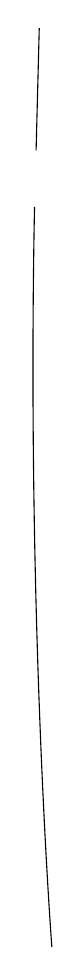
\begin{tikzpicture}[x=1cm,y=1cm]
\draw (0,0) -- (-0.04,-1.55);
\draw (-0.06,-2.27) .. controls (-0.14,-6.3) and (0.04,-10.0) .. (0.16,-11.67);
\end{tikzpicture}}}

We have a group $\Gamma$ of \unsure{automorphisms} of $\mathcal X$ ($\Gamma$ profinite in the profinite case --- to do things properly we should spell out the reasonable hypotheses to be made to take account of the profinite topology of $\Gamma$\ldots). We put
\[
\Pi=\Pi_1(\mathcal X,x_0),\quad \mathcal M=\Pi_1(\mathcal X,\Gamma;x_0)\qquad\text{hence}
\]
\inserted{\diagram{\begin{tikzcd}[column sep=large]
{(*)}\quad 1 \arrow[r,no head] & \Pi \arrow[r,no head] & \mathcal M \arrow[r,no head] & \Gamma \arrow[r] & 1
\end{tikzcd}}}
we give ourselves a quotient $M$ of $\Pi$, \deleted{\unsure{a}} by a normal subgroup \uline{in $\mathcal M$}, \unsure{or} what amounts to the same thing a quotient of $\Pi_{\mathrm{ab}}=\Pi/[\Pi,\Pi]$ stable under the action of $\Gamma$, \deleted{for}\inserted{hence} a \deleted{$\widetilde{\mathcal M}=\mathcal M/$} quotient extension of $(*)$,
\[
(287)\qquad
\diagram{\begin{tikzcd}[column sep=large]
1 \arrow[r] & M \arrow[r,no head] & \widetilde{\mathcal M} \arrow[r,no head] & \Gamma \arrow[r,no head] & 1
\end{tikzcd}}
\]
where $M$ is \unsure{commutative|commutative} so $\Gamma$ operates on $M$.

We are interested in the category of coverings \deleted{$\unsure{M_{\mathcal X}}$-torsors $\mathcal X'_0$ \unsure{over}} $\mathcal X'$ of $(\mathcal X,\Gamma)$, satisfying the conditions

\margin{129}

\begin{center}
\small
129\\
\texttt{https://grothendieck.umontpellier.fr}\\
Université de Montpellier, UMR CNRS 5149, Case courrier 051, Place Eugène Bataillon\\
34095 Montpellier cedex 5 - France
\end{center}

\scanpage{131}
\mspage{713}

Following : after forgetting the operations of $\Gamma$, we find a \inserted{connected} Galois covering \inserted{\unsure{(and even abelian)}} of $\mathcal X$, corresponding to the quotient group $M$ of $\Pi=\Pi_1(\mathcal X,x_0)$ --- so that $\mathcal X'$ becomes in a natural way a torsor under $M_{\mathcal X}$.
\margin{\figure{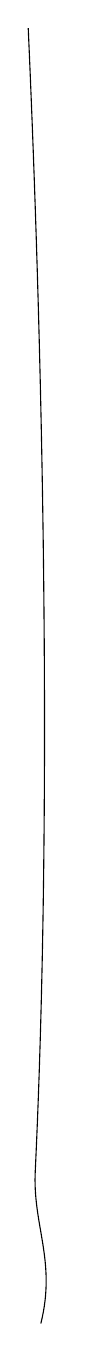
\begin{tikzpicture}[x=1cm,y=1cm]
\draw (0,0) .. controls (0.2,-4.5) and (0.3,-10.0) .. (0.09,-14.5) .. controls (0.05,-15.2) and (0.36,-15.65) .. (0.16,-16.45);
\end{tikzpicture}}}
The functor
\[
\mathcal X'\longmapsto\mathcal X'(x_0)\qquad\text{(fiber at $x_0$)}
\]
from the category of these $\mathcal X'$ to the category of sets, in fact goes to the sets $E$ equipped with the following structures

\noindent a) $E$ is an $M$-torsor, and as such gives rise to an extension
\diagram{\begin{tikzcd}[column sep=large]
1 \arrow[r,no head] & M \arrow[r] & \operatorname{Aff}(E) \arrow[r] & \operatorname{Aut}(M) \arrow[r,no head] & 1
\end{tikzcd}}
hence an \unsure{induced} subextension
\[
(288)\qquad
\diagram{\begin{tikzcd}[column sep=large]
1 \arrow[r,no head] & M \arrow[r,no head] & \operatorname{Aff}_{\Gamma}(E) \arrow[r] & \widetilde\Gamma \arrow[r,no head] & 1
\end{tikzcd}}
\]
where
\[
\widetilde\Gamma=\operatorname{Im}(\Gamma\longrightarrow\operatorname{Aut}(M)).
\]

\noindent b) We have a homomorphism of extensions
\[
(289)\qquad
\diagram{\begin{tikzcd}[column sep=large,row sep=large]
1 \arrow[r,no head] & M \arrow[r,no head] \arrow[d,Rightarrow,"\mathrm{id}"] & \widetilde{\mathcal M} \arrow[r,no head] \arrow[d,"\Theta_{\widetilde{\mathcal M}}"] & \Gamma \arrow[r,no head] \arrow[d,"\mathrm{can}"] & 1 \\
1 \arrow[r,no head] & M \arrow[r,no head] & \operatorname{Aff}_{\Gamma}(E) \arrow[r,no head] & \widetilde\Gamma \arrow[r,no head] & 1
\end{tikzcd}}\qquad .
\]
The category of the $\mathcal X'$ (with isomorphisms\ldots) is equivalent to that of \deleted{$\unsure{M}$} pairs $(E,\Theta_{\widetilde{\mathcal M}})$, where $E$ is an $M$-torsor, and $\Theta_{\widetilde{\mathcal M}}$ a homomorphism of extensions (289).

\margin{130}

\begin{center}
\small
130\\
\texttt{https://grothendieck.umontpellier.fr}\\
Université de Montpellier, UMR CNRS 5149, Case courrier 051, Place Eugène Bataillon\\
34095 Montpellier cedex 5 - France
\end{center}

\scanpage{132}

The automorphisms of an object $\mathcal X'$ correspond to ``translations'' by elements of $M^\Gamma$\inserted{$=\operatorname{Cent}(\widetilde{\mathcal M})$}, (\unsure{in} the terms of $E,\Theta_{\widetilde{\mathcal M}}$) to translations of $E$ by \deleted{such \unsure{elements|elements}} elements of $M^\Gamma$, \deleted{which in \unsure{so far}}\inserted{(in so far} as elements of $\operatorname{Aff}_{\Gamma}(E)$ they are central, and by conjugating by these elements we find the \uline{same} homomorphism $\Theta_{\widetilde{\mathcal M}}$\ldots).
\margin{\figure{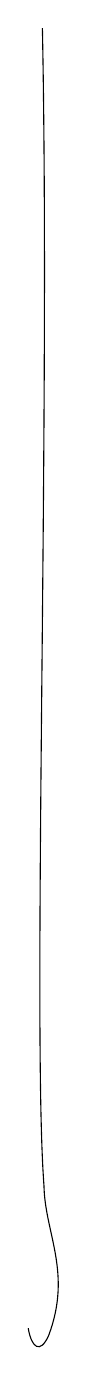
\begin{tikzpicture}[x=1cm,y=1cm]
\draw (0,0) .. controls (0.10,-5.0) and (-0.13,-12.7) .. (0.02,-14.7) .. controls (0.03,-15.3) and (0.38,-15.8) .. (0.08,-16.6) .. controls (-0.03,-16.85) and (-0.14,-16.75) .. (-0.18,-16.51);
\end{tikzpicture}}}
The isomorphism classes of such \unsure{elements} \deleted{\unsure{identify}}\inserted{\unsure{correspond}} one-to-one to the $M$-conjugacy classes of splittings of the extension (287) of $\Gamma$ by $\widetilde{\mathcal M}$. In precise terms, to an $(E,\Theta_{\widetilde{\mathcal M}})$ is associated \unsure{canonical|canonically} a \deleted{$\unsure{M}$} homomorphism of $M$-sets
\[
(290)\qquad
\diagram{\begin{tikzcd}[column sep=large]
E \arrow[r] & \operatorname{Scind}(\widetilde{\mathcal M}\ \unsure{\text{extension}}\ \text{of }\Gamma\ \text{by }M)
\end{tikzcd}}
\]
whose image is the conjugacy class \unsure{describing} the isomorphism class under consideration. \deleted{\unsure{The image}}\inserted{The homomorphism} (290) \unsure{is|of} factored through $M^\Gamma\backslash E$ as a \uline{monomorphism}
\[
(291)\qquad
\diagram{\begin{tikzcd}[column sep=large]
M^\Gamma\backslash E \arrow[r,hook] & \operatorname{Scind}(\widetilde{\mathcal M}\ \text{extension of }\Gamma\ \text{by }M)
\end{tikzcd}},
\]
and if $M^\Gamma=0$, we see that $E$ is canonically reconstructed from the class of

\margin{131}

\begin{center}
\small
131\\
\texttt{https://grothendieck.umontpellier.fr}\\
Université de Montpellier, UMR CNRS 5149, Case courrier 051, Place Eugène Bataillon\\
34095 Montpellier cedex 5 - France
\end{center}

\scanpage{133}
\mspage{714}

conjugacy under consideration. The \inserted{(affine)} operation of $\widetilde{\mathcal M}$ on $E$ \inserted{(defined by $\Theta_{\widetilde{\mathcal M}}$)} is none other than the operation \deleted{of} \inserted{(\unsure{induced} by the)} conjugation on \inserted{the set} of splittings (which of course does not take one out of an $M$-conjugacy class, even when conjugating by arbitrary elements of $\widetilde{\mathcal M}$).
\margin{\figure{
\begin{tikzpicture}[x=1cm,y=1cm]
\draw (0,0) .. controls (-0.03,-1.65) and (0.07,-3.9) .. (0.21,-5.7);
\end{tikzpicture}}}

\uline{Corollary} Suppose we have
\[
(292)\qquad \underbrace{H^0(\widetilde\Gamma,M)}_{M^\Gamma}=H^1(\widetilde\Gamma,M)=0
\]
i.e. that \deleted{\unsure{all|all}} two splittings of a trivial extension of $\widetilde\Gamma$ by $M$ are conjugate by a unique element of $M$. This implies \inserted{therefore (because of $M^\Gamma=\unsure{\{0\}|0}$)} that the category of the $\mathcal X'$, or again that of the pairs $(E,\Theta_{\widetilde{\mathcal M}})$, is rigid, \deleted{Then the classes} \inserted{i.e. an object is known up to an isomorphism} which is unique when we know its isomorphism class. This being so, the isomorphism classes in question \deleted{correspond}\inserted{(i.e. the classes} of \deleted{$M$-\unsure{conjugation|conjugation}} conjugacy of the splittings of \deleted{one-to-one} the extension $\widetilde{\mathcal M}$ of $\Gamma$ by $M$) correspond one-to-one to the quotient groups $\widetilde{\widetilde{\mathcal M}}$
\margin{\figure{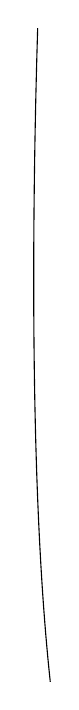
\begin{tikzpicture}[x=1cm,y=1cm]
\draw (0,0) .. controls (-0.06,-1.95) and (-0.12,-5.7) .. (0.16,-8.3);
\end{tikzpicture}}}

\margin{132}

\begin{center}
\small
132\\
\texttt{https://grothendieck.umontpellier.fr}\\
Université de Montpellier, UMR CNRS 5149, Case courrier 051, Place Eugène Bataillon\\
34095 Montpellier cedex 5 - France
\end{center}